\section{Introduction}
What this guide is about, how to use this guide.

\subsection{Conventions used in this Guide}
\begin{figure}[h!] % h - here
	\centering
	\includesvg[
		inkscapelatex=false,
		width = 32pt
	]{2d.svg}
	\caption{2D symbol}
	\label{fig:2d_icon}
\end{figure}
\noindent
The element in Figure \ref{fig:2d_icon} signifies that a tool can be used in 2D views.\newline

\begin{figure}[h!] % h - here
	\centering
	\includesvg[
		inkscapelatex=false,
		width = 32pt
	]{3d.svg}
	\caption{3D symbol}
	\label{fig:3d_icon}
\end{figure}
\noindent
The element in Figure \ref{fig:3d_icon} signifies that a tool can be used in 3D views.\newline

\begin{figure}[h!] % h - here
	\centering
	\includesvg[
		inkscapelatex=false,
		width = 55pt
	]{hint.svg}
	\caption{Hint symbol}
	\label{fig:hint_icon}
\end{figure}
\noindent
The element in Figure \ref{fig:hint_icon} signifies a tip or hint.\newline

\begin{figure}[h!] % h - here
	\centering
	\includesvg[
		inkscapelatex=false,
		width = 55pt
	]{irreversible.svg}
	\caption{Irreversible symbol}
	\label{fig:noundo_icon}
\end{figure}
\noindent
The element in Figure \ref{fig:noundo_icon} signifies to be cautious because a operation may not be undone.\pagebreak

\begin{figure}[h!] % h - here
	\centering
	\includesvg[
		inkscapelatex=false,
		width = 55pt
	]{performance.svg}
	\caption{Performance symbol}
	\label{fig:performance_icon}
\end{figure}
\noindent
The element in Figure \ref{fig:performance_icon} signifies that a operation may use a lot of resources.\newline

\begin{figure}[h!] % h - here
	\centering
	\includesvg[
		inkscapelatex=false,
		width = 55pt
	]{plugin.svg}
	\caption{Plugin symbol}
	\label{fig:plugin_icon}
\end{figure}
\noindent
The element in Figure \ref{fig:plugin_icon} signifies that a tool may only be available after installing a third party plugin.\newline

\noindent
If you are already familiar with 3D Slicer and want to start with the segmentation right away, skip to page \pageref{qsg} for the Quick Start Guide.

\subsection{Installation}
Basic installation instructions for 3D Slicer:
\begin{enumerate}
	\item Browse to: \url{https://download.slicer.org}
	\item Download the installer of the latest stable release\footnote{Version 5.6.2 at the time of writing this document} for your Operating System
	\item Run the installer and follow its instructions
\end{enumerate}

\subsubsection{Installation on macOS}
On macOS, 3D Slicer can be installed in two different ways:\newline\newline
Either via the provided package on the downloads page, or via Homebrew: \url{https://formulae.brew.sh/cask/slicer}\newline
For the conventional installation refer to the 3D Slicer wiki: \url{https://slicer.readthedocs.io/en/latest/user_guide/getting_started.html#mac}

\subsubsection{Installation on Linux}
3D Slicer ships with all its dependencies on Windows and macOS.\\
On Linux it is required to install some dependencies via your distributions package manager.\\
The 3D Slicer wiki gives information about required packages and their respective names on different distributions:
\url{https://slicer.readthedocs.io/en/latest/user_guide/getting_started.html#linux}.\\
To make this process easier, this guide provides a distrobox manifest file (see page: \pageref{code:distrobox-manifest}).
Which allows the user to create a Linux container containing all necessary dependencies without polluting the host system.\newline\newline
To run 3D Slicer via the container run:
\inputminted[
	%fontsize=\footnotesize, % set text size
	stripnl, % strip leading newlines
	numbers=left, % display line numbers on the left
	breaklines % break lines after spaces if necessary
]{sh}{./code/runSlicer.sh}

\subsection{System Requirements\cite{fedorov3DSlicerImage2012}}
Note: as of \today
\subsubsection{Official supported operating systems}
\begin{itemize}
	\item Windows: 10 or 11
	\item macOS: 11 or later
	\item Linux:
	      \begin{itemize}
		      \item Ubuntu 20.04 or later
		      \item Debian 10 or later
		      \item Fedora 35 or later
		      \item CentOS 7 or later
	      \end{itemize}
\end{itemize}

\subsubsection{Hardware requirements}
\begin{itemize}
	\item Memory: At least 4 Gigabytes, more is strongly recommended.\\ The 3D Slicer wiki mentions needing about 10 times more memory than the amount of data you plan to load.\\ 3D Slicer on its own uses about 456 Megabytes of RAM. After loading a 26.17MiB Dataset it consumes about 614 MB.
	\item \gls{cpu}: 3D Slicer uses multi-threading for some calculation and will thus benefit from a multi-core CPU.
	\item \gls{gpu}: A dedicated GPU is recommended but not required as 3D Slicer only uses it for interactive volume rendering. If you restrict your usage to the 2D views, you will hardly ever use your graphics card.
\end{itemize}

\subsubsection{Hardware recommendations}

\begin{itemize}
	\item Input devices: 3D Slicer supports Mice, touchpads, pens, graphic tablets and OpenVR headsets. The easiest input method though is a 3 button Mouse with a mouse wheel.
	\item Internet connection: for downloading extensions, online documentation and sample data sets.
	\item \gls{vram}: for interactive volume rendering it is recommended to have more GPU texture memory than the data set you plan to load.
	\item A large display or monitor with a decent screen resolution. I would recommend at least a 14 inch screen with 1920x1080 resolution or larger.
\end{itemize}


\subsection{Interface and Usage}
Upon first launch you will be greeted by the 3D Slicers welcome screen (see: Figure \ref{fig:slicerWelcome})
\begin{figure}[h!] % h - here
	\centerline{
		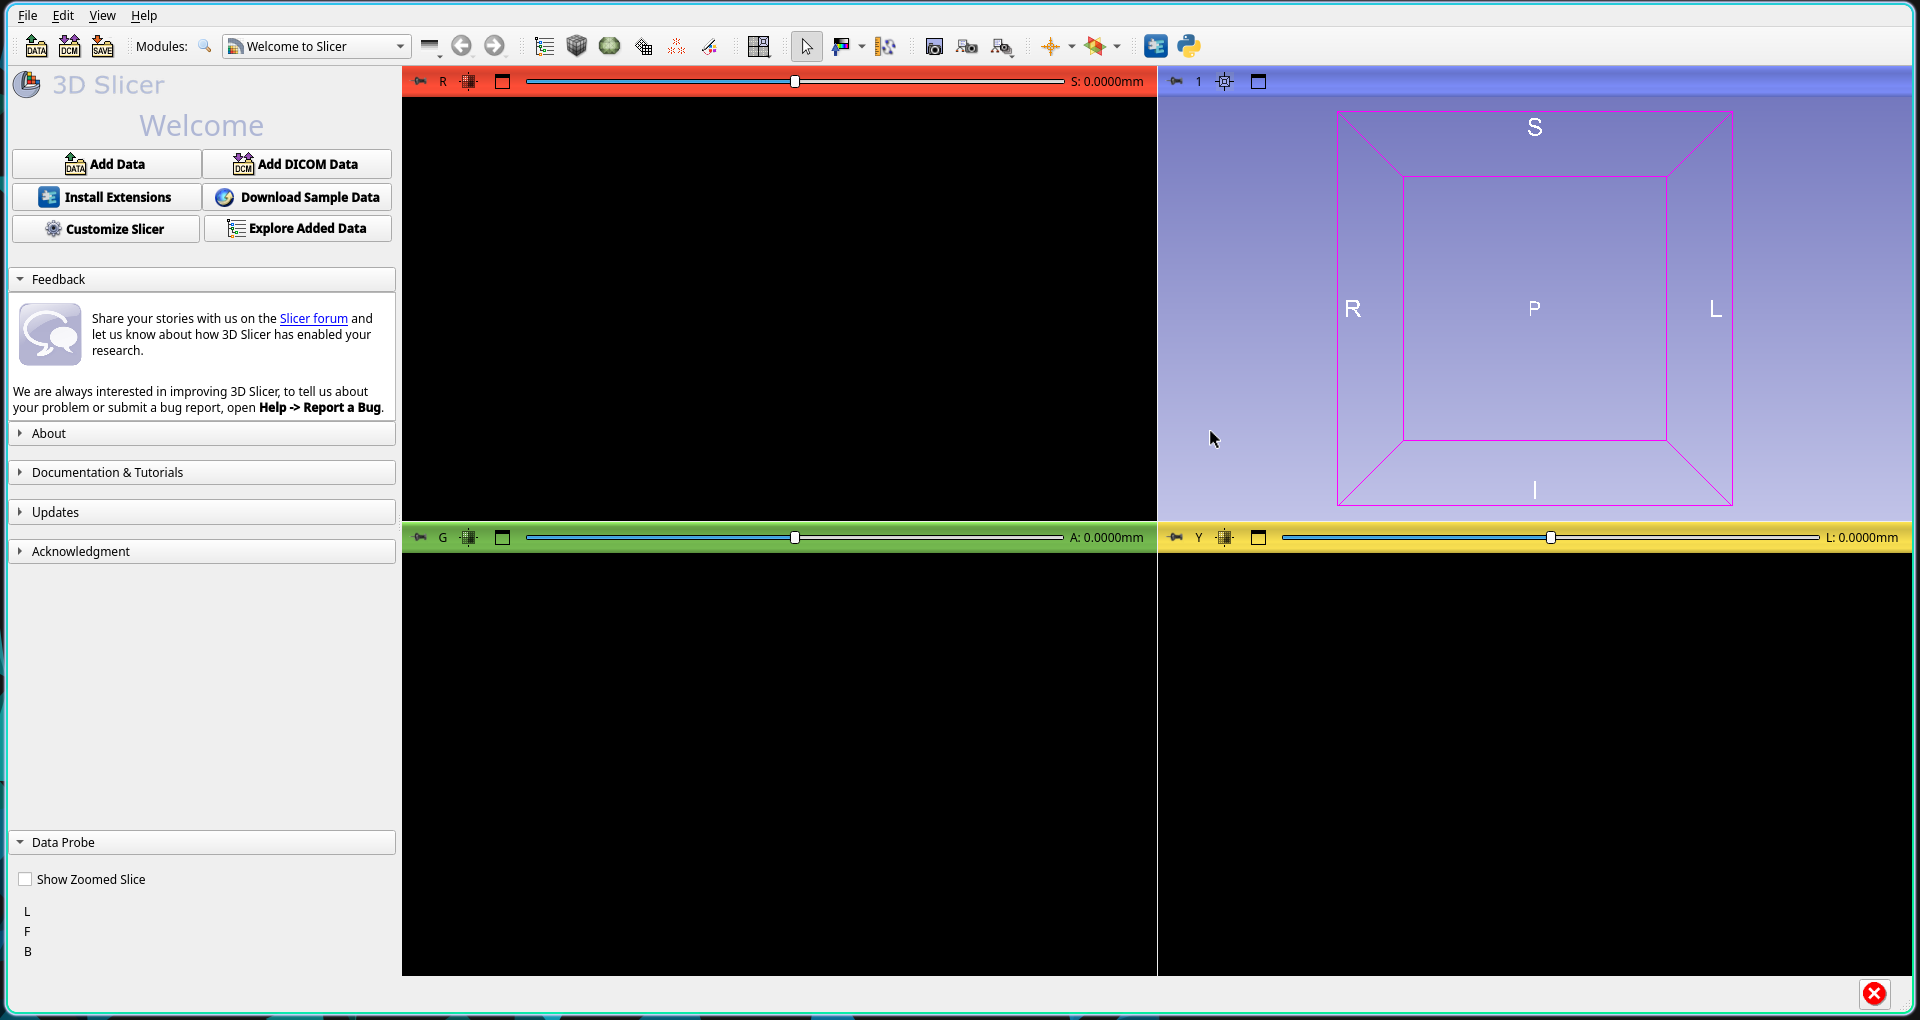
\includegraphics[
			% scale=0.2
			width=0.95\paperwidth
		]{slicerWelcome.png}}
	\caption{3D Slicer welcome screen}
	\label{fig:slicerWelcome}
\end{figure}

The welcome screen has some quick links to useful modules like load data and download datasets. (TODO)
\pagebreak
\begin{figure}[h!] % h - here
	\centerline{ % center a single element on page, from: https://tex.stackexchange.com/a/4438
		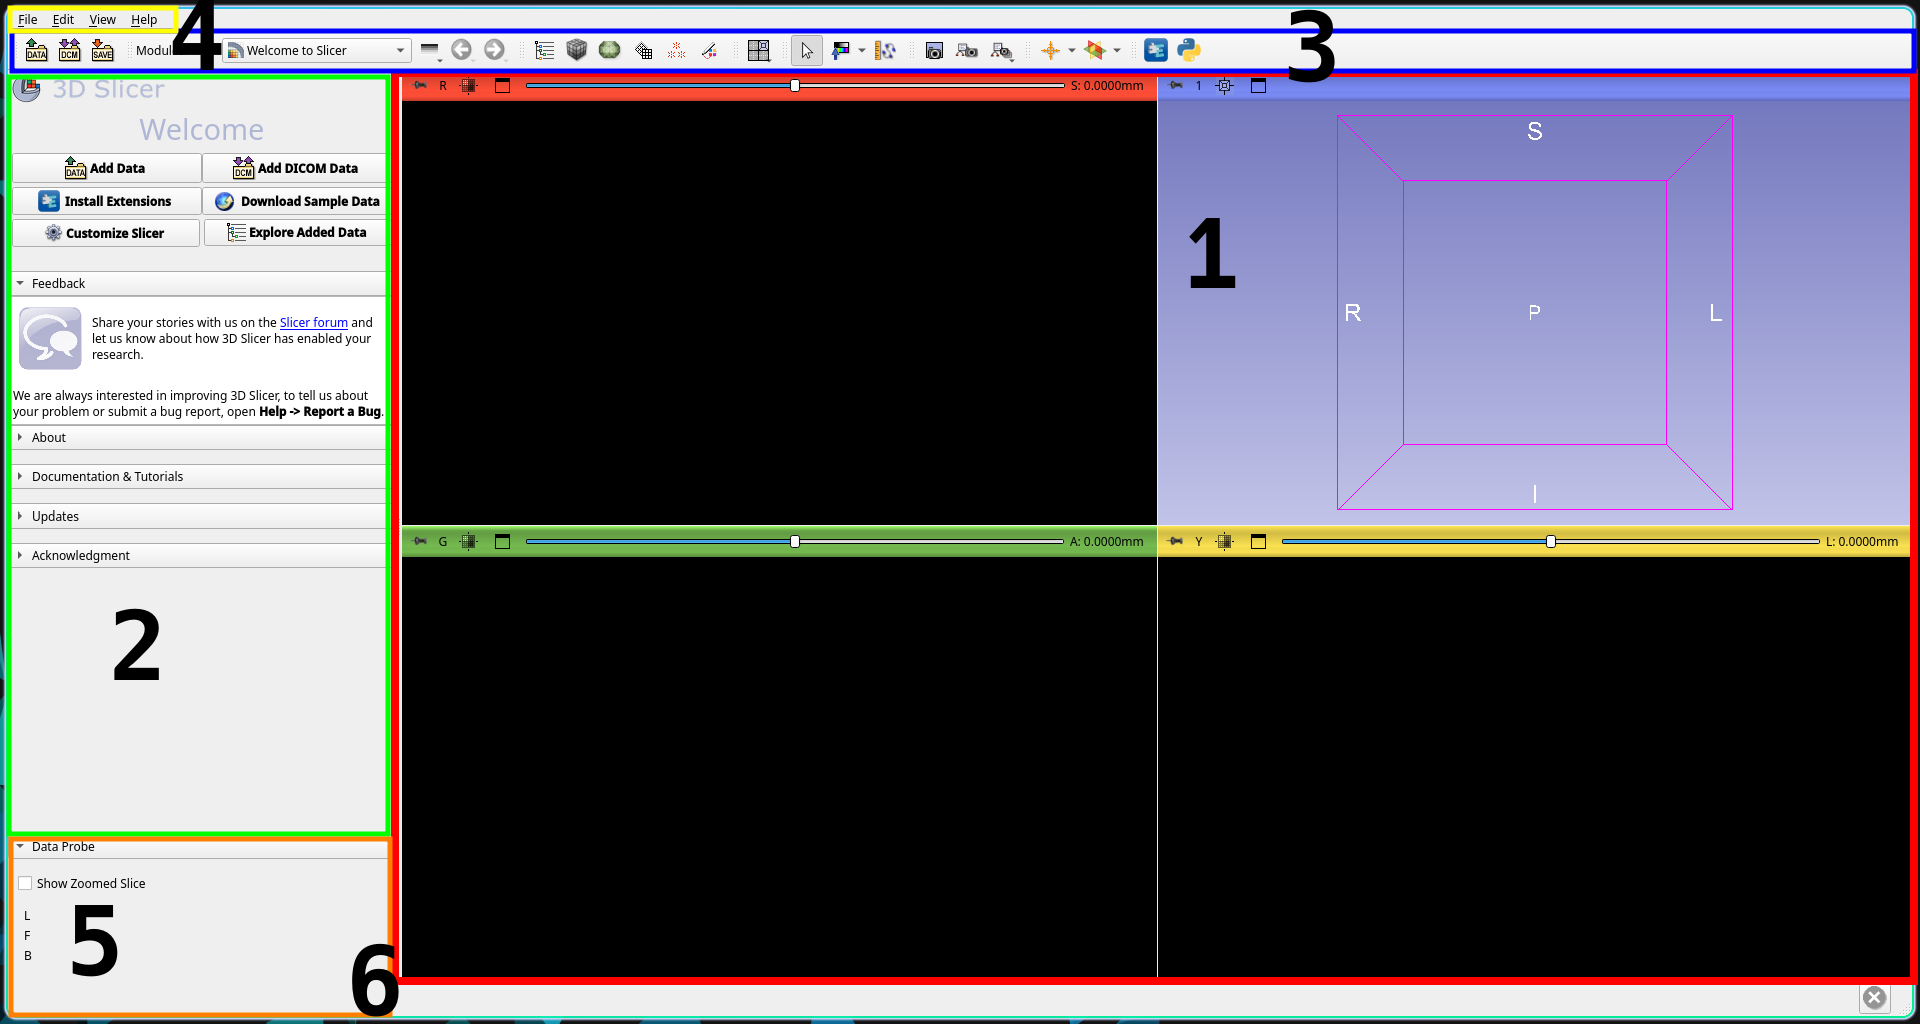
\includegraphics[
			% scale=0.2
			width=0.95\paperwidth
		]{slicerWelcomeMarked1.png}}
	\caption{3D Slicer window}
	\label{fig:slicerView}
\end{figure}

\noindent
The 3D Slicer window consists of several areas, which provide different tools to interact with the program.
A quick overview of these areas is provided by Figure \ref{fig:slicerView}:
\begin{enumerate}
	\item View area
	\item Module panel
	\item Toolbar
	\item Application menu
	\item Data probe
	\item Status bar
\end{enumerate}



\pagebreak
\subsubsection{ The view area }
By default 3D Slicer shows the view area (see Figure \ref{fig:4upview}) with three 2D slice views and the interactive 3D view at the top right.\\
\noindent
\begin{figure}[h!] % h - here
	\centerline{ % center a single element on page, from: https://tex.stackexchange.com/a/4438
		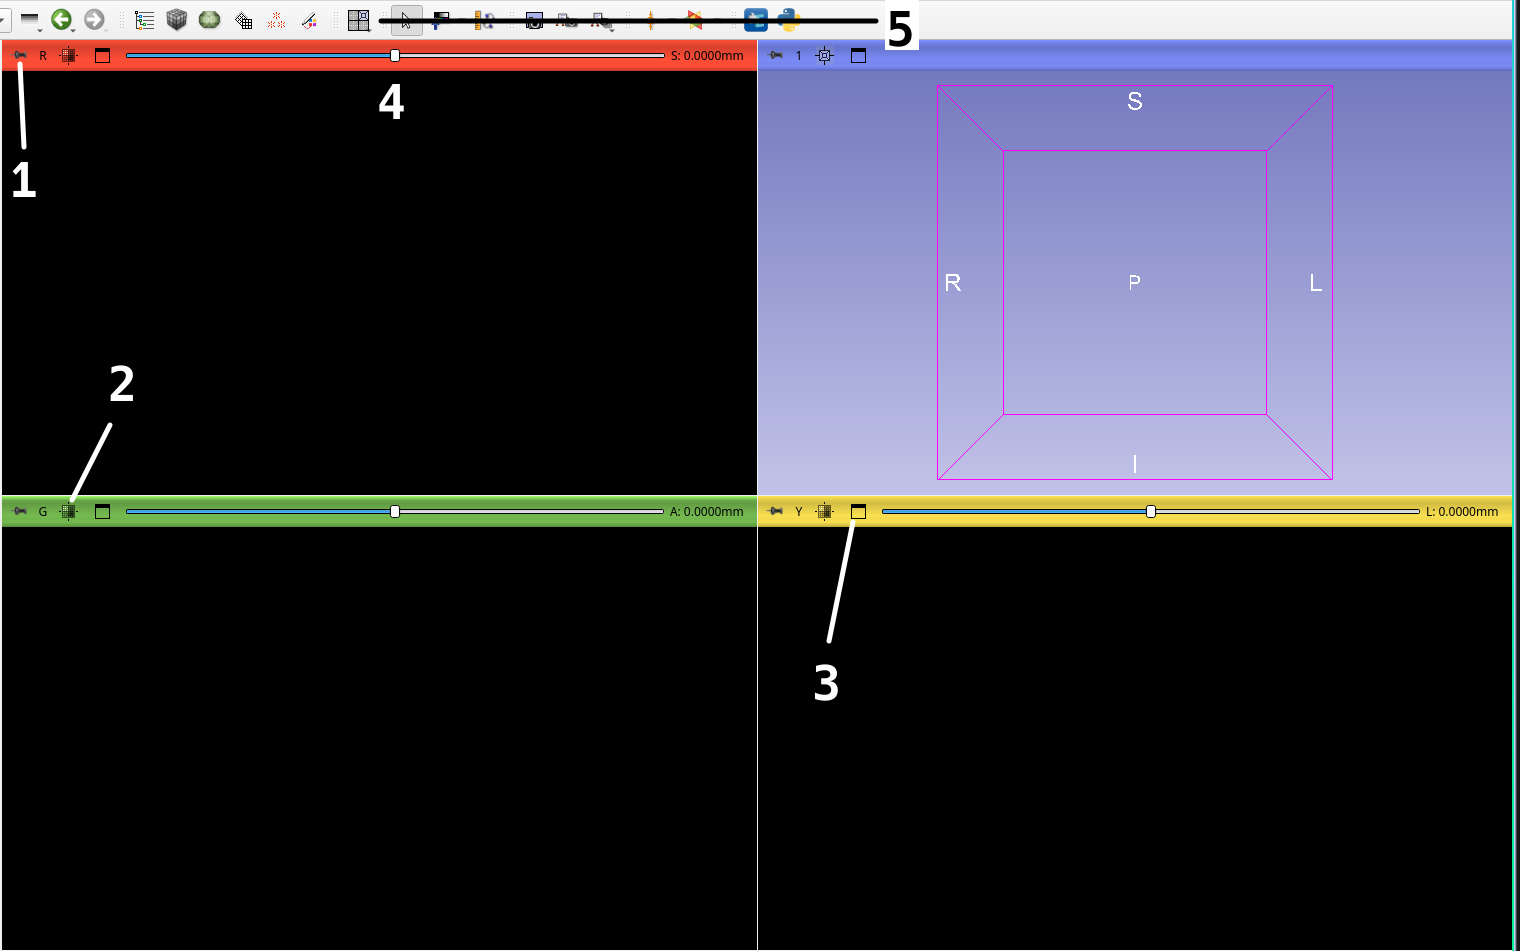
\includegraphics[
			% scale=0.2
			width=0.95\paperwidth
		]{view.png}}
	\caption{3D Slicer view area}
	\label{fig:4upview}
\end{figure}

\noindent
3D Slicer calls this the 'Four-up' view.\\

\noindent
There is a numerous amount of view presets to choose from by clicking on the 'change view' option in the toolbar: Figure \ref{fig:4upview}:5.\\

\noindent
Each slice view has its own scroll bar (Figure \ref{fig:4upview}:4).
The number on the right end of the scroll bar shows by how much a single tick scrolls through the dataset.
In other words: it shows the slice thickness of the view.\\
\noindent
Scrollbar controls:
\begin{itemize}
	\item left click and drag the scrollbar
	\item mouse wheel
	\item 'B' and 'F' Keys
	\item up, down, left and right arrow keys
\end{itemize}

\noindent
To maximize a single slice view, click on the 'Maximize view' button (Figure \ref{fig:4upview}:3). Click it again to return to the previous layout. Double left-clicking on the slice has the same effect.\\

\noindent
'Reset \gls{fov}' can be used to reset the zoom level and shift the slice into its isocenter (Figure \ref{fig:4upview}:2). The 'R' key has the same effect.\\

\noindent
The pin icon (Figure \ref{fig:4upview}:1) brings up a submenu:

\noindent
This layout can be customized to a great extent if needed, but before you start customizing the view area, check if a pre-made view layout covers your needs.
Use the view layout selection menu to change the currently displayed layout. This menu also comes in handy if you changed the layout and quickly want to change it back without manually undoing all your customizations.
Each 2D view area has its own scroll bar, (TODO)

\subsubsection{Zitate sind für wissenschaftliche Arbeiten unerlässlich}

Für das Arbeiten mit Quellen, empfehle ich Zotero (oder Mendeley).
Natürlich geht's auch die Quellen direkt aus zB Scholar im \textit{bibtex} Format ins Verzeichnis (= *.bib-Datei) zu kopieren.

\subsubsection{Auf Grafiken kann selten verzichtet werden}
Grafiken

\subsubsection{Formeln sind in der angewandeten Informatik seltener anzutreffen}
Die folgende Formel ist als eigenständige Formel nummeriert:
\begin{equation}
	\frac{\partial^2 }{\partial x^2}  % Online Formeleditor (google!) wirkt Wunder!
\end{equation}

Formeln können aber auch direkt in den Text $\frac{\partial^2 }{\partial x^2}$, was allerdings schwer zu lesen ist.
Für die Formeln in \LaTeX gibt's im Web eigene \textit{Cheat Sheets}, schließlich wurde es extra für den Formelsatz entwickelt.


\subsubsection{Tabellen gehören ohne Gitternetzlininen (booktabs Stil)}
Tabellen im Booktabs Stil sind professioneller gestaltet und lenken nicht durch Gitternetzlinien ab. Das ist gut so, denn welche Daten haben es schon verdient, ihr Leben hinter Gittern zu verbringen?
Zum Glück, gibt's dafür Online Editoren, denn von der Usability her, ist das händische Setzen einer Tabelle eine Katastrophe.

% \begin{table}[h]

% \centering
% \begin{tabular}
%\toprule
% ID & \multicolumn{1}{l}{Farbe} & \multicolumn{1}{l}{Anteil} \\ \midrule
% 1  & rot                       & 255                        \\
% 2  & grün                      & 255                        \\
% 3  & blau                      & 0                          \\ \bottomrule
% \end{tabular}
% \caption{Tabellen werden fallweise auch oben beschriftet. Dann einfach die caption im Quellcode an die richtige Stelle verschieben.}
% \end{table}


\subsubsection{Programmcode darf nur auszugsweise in die Arbeit}

Eigentlich gehören komplette Codelistings in den Anhang.
Wenn aber in der Arbeit zB ein Algorithmus erläutert werden soll, dann gehört das natürlich direkt in die Arbeit.

Verbatim ist dabei die einfachste Variante für Programmcode.
Ausgefeilter geht's dann zB mit lstlistings zur Sache, wo auch Syntax Highlighting vorgenommen werden kann. \\

Müssen Klassen-/Methoden-/Variablennamen im Fließtext erwähnt werden, bietet sich ein Inline-Verb-Block an, mit dem kann auf eine \verb|Class1.Method1()| Bezug genommen werden, ohne dass diese als zu lesendes Wort missverstanden wird. %PHR

\subsubsection{Wie man mit Aufzählungen verfährt}

Nummerierte Aufzählungen werden nur dann eingesetzt, wenn wirklich eine Reihenfolge vorliegt.
Kann auch geschachtelt werden (siehe Beispiel).

\begin{enumerate}
	\item Erster Schritt
	\item Zweiter Schritt
	      \begin{enumerate}
		      \item erster Subschritt zu Schritt zwei
		      \item zweiter Subschritt zu Schritt zwei
	      \end{enumerate}
	\item Dritter Schritt
\end{enumerate}

Aufzählungen, die keine zwingende Reihenfolge wiedergeben werden durch \textit{Bullet Points} formatiert.
In folgenden Beispiel wird auf Schachtelung verzichtet, obwohl sie ohne weiteres möglich wäre.

\begin{itemize}
	\item grüner Tee
	\item schwarzer Tee
	\item weisser Tee
	\item aromatisierter Tee
	\item Kräuterteee
\end{itemize}

\subsubsection{Ein paar persönliche Tipps zum Arbeiten - bitte ohne Scheu ergänzen!}

Jeden Satz in einer eigenene Zeile - das hab ich zwar schon erwähnt, ist für mich aber eine wirkliche Hilfe, wenn man sich einmal daran gewöhnt hat.

Hervorhebungen im Text \textit{nie} mit fett oder unterstrichen, sonderm \textit{immer} mit kursivem Text.
Das kriegt man entweder durch \textit{textit} hin oder \textit{emph}

(Harte) Zeilenumbrüche macht man mit einem doppelten Backslash, Absatzumbrüche hingegen durch mehr als 2 Absatzschaltungen im Quelltext.
Die Anzahl der Leerzeilen wird dabei nicht berücksichtigt, was zur schöneren Strukturierung des Quelltexts beiträgt.

Kommentare helfen, nichts zu vergessen.
% nicht vergessen!

Quick \& Dirty -- die Rohversion der Arbeit sollte möglichst zügig verfasst werden.
Das hilft, den roten Faden nicht zu verlieren.
Überarbeiten, umformulieren, Grafiken usw einfügen und überhaupt verschönern kann man später.

Warnungen (gelbes Dreieck) in Overleaf betreffen meist \textit{overfull boxes} d.h. der Text ist zu lang.
Bis zur finalen Version können diese ignoriert werden.
Fallen sie dann tatsächlich ins Gewicht (nur dann!) kann man versuchen, diese durch manuelle Silbentrennung hinzukriegen.

Querverweise verwenden die \textit{labels} zB bei Grafiken oder Tabellen und werden mit \textit{ref} oder \textit{pageref} eingefügt.

Fast nicht zu entdecken: die kleinen Dreiecke neben den Zeilennummern in Oveleaf.
Damit kann man den Bereich \textit{einfalten}, was zur Übersicht beiträgt.

Wenn man in der Vorschau doppelt in den Text klickt, springt man im Editor auf die Stelle im LaTeX-Quellcode.

Wenn man länger AFK war, dann kann's sein, dass man aus Overleaf abgemeldet ist.
Bei mir hat's noch NIE funktionert, sich über Button neu zu verbinden - es war immer ein Aussteigen - Einsteigen notwendig.

Wer sich von den überwältigenden Möglichkeiten mit LaTeX beeindrucken lassen will, googelt nach \textit{Tikz}.
Da gibt's dann fast Nix, was es nicht gibt.

Grundsätzlich ist bei der Arbeit mit \LaTeX Google ein guter Freund.
Die Community ist riesig und was man nicht in der sehr guten Hilfe von Overleaf findet, hat in den allermeisten Fällen jemand anderer schon gepostet.








